\documentclass[a4paper,12pt,reqno]{article}

\usepackage{../styledoc19}

\begin{document} % конец преамбулы, начало документа
	
	\itsHSE
	\academicTeacher{Преподаватель департамента \vfill программной инженерии  факультета компьютерных наук}
	{М. К. Горденко}
	
	\projectName{IOS-ПРИЛОЖЕНИЕ <<СОЦИАЛЬНАЯ СЕТЬ ДЛЯ СОТРУДНИКОВ НИУ ВШЭ>>}
	
	\titleList{Техническое задание}{RU.17701729.04.03-01 ТЗ 01-1-ЛУ}
	\par\vspace{60mm}
	\nameOfAuthor{БПИ174}{Д. Ю. Редникина}
	\tabForFirstPage
	
						\newpage
	
	\pagestyle{fancy}
	\lhead{УТВЕРЖДЕН \newline
	 	RU.17701729.04.03-01 ТЗ 01-1-ЛУ}
	\vspace*{9cm}
	\begingroup
	\centering
	\projectName{IOS-ПРИЛОЖЕНИЕ <<СОЦИАЛЬНАЯ СЕТЬ ДЛЯ СОТРУДНИКОВ НИУ ВШЭ>>}
	\titleListTwo{Техническое задание}{RU.17701729.04.03-01 ТЗ 01-1}
	\listNumber{26}
	
	\endgroup
	\vspace{8cm}
	\tabForFirstPage
	\vspace*{\fill}
	
	
						\newpage
	\lhead{ }
	\chead{\vfill \thepage \vfill  RU.17701729.04.03-01 ТЗ 01-1 }
	\rhead{ }
	\cfoot{ }
	%delete this if you are not writing a TZ
	\cfoot{\tabForTZ}
	\tableofcontents
	\newpage
	\section{Введение}
	\subsection{Наименование программы}
	\subsubsection{Наименование программы на русском языке}
iOS-приложение <<Социальная сеть для сотрудников НИУ ВШЭ>>
\subsubsection{Наименование программы на английском языке}
iOS application <<Social network for HSE staff>>
	\subsection{Краткая характеристика области применения}
	% ОБЛАСТЬ ПРИМЕНЕНИЯ

НИУ ВШЭ очень большой вуз с кампусами в разных городах России. Преподавателям сложно общаться между собой, узнавать последние новости, связанные с написанием статей, научно-исследовательской деятельностью коллег. Разрабатываемая программа позволит наладить взаимодействие преподавателей и будет способствовать развитию научной деятельности и коммуникации между факультетами и кампусами университета.

Задача социальной сети заключается в обеспечении коммуникации, обмене актуальной научной и общеуниверситетской информацией, знакомстве научных работников и преподавателей с разных факультетов и кампусов. 

Разрабатываемая программа является прекрасной площадкой для начала исследований, обсуждения научных работ, общения по научным и университетским тематикам для сотрудников университета НИУ ВШЭ.
	\newpage
	\section{Основания для разработки}
	\subsection{Документы, на основании которых ведется разработка}
	
	
	Приказ декана факультета компьютерных наук Национального Исследовательского университета <<Высшая школа экономики>> № 2.3-02/1012-0 2 от 10.12.18.
	
	\subsection{Наименование темы разработки}
	
	Наименование темы разработки – iOS-приложение <<Социальная сеть для сотрудников НИУ ВШЭ>>  (iOS application <<Social network for HSE staff>>).


 Программа выполняется в рамках темы курсовой работы в соответствии с учебным планом подготовки бакалавров по направлению 09.03.04 «Программная инженерия» Национального исследовательского университета «Высшая школа экономики», факультет компьютерных наук.
	
	\newpage 
	\section{Назначение разработки}
	 
	\subsection{Функциональное назначение}
	Программа применяется как средство коммуникации между сотрудниками НИУ ВШЭ. Сервис также позволяет сотрудникам НИУ ВШЭ координировать совместные исследования и проекты научного характера. Приложение предоставляет доступ к общению посредством сообщений, дает возможность делиться новостями с помощью публикации постов. Также приложение дает возможность фильтровать новости по интересущим темам. 

	\subsection{Эксплуатационное назначение}
	% ЭКСПЛУАТАЦИОННОЕ НАЗНАЧЕНИЕ

Программа будет использоваться как средство общения и огранизации работы над совместными научными проектами между сотрудниками с одного или разных направлений/ факультетов/ кампусов. 


Таким образом, программный продукт позволит решить проблему коммуникации между факультетами, кампусами НИУ ВШЭ и даст возможность наладить взаимодействие между преподавателями университета, будет способствовать развитию научной деятельности между разными факультетами и кампусами.
	
						\newpage
	\section{Требования к программе}
	\subsection{Требования к функциональным характеристикам}
	\subsubsection{Требования к составу выполняемых функций}\label{subsec:requirements}
	
	% требования
% dyurednikina
% version 1.2
% last modified 7.05.2019


Программа выполняется в рамках темы курсовой работы в соответствии с учебным планом подготовки бакалавров по направлению 09.03.04 «Программная инженерия» Национального исследовательского университета «Высшая школа экономики», факультет компьютерных наук.

Разработка требований велась совместно с командой и заказчиком в рамках предмета <<Групповая динамика и коммуникации в программной инженерии>>



\textit{Состав команды}:
\begin{itemize}
	\item Анна Михалева - android-developer;
	\item Константин Манежин - web-developer;
	\item Илья Костюченко - backend-developer;
	\item Дарья Редникина - iOS-developer;
\end{itemize}


\textit{Заказчик}:
\begin{itemize}
	\item Девятьярова Анна Дмитриевна, Факультет бизнеса и менеджмента/ 
	Кафедра управления человеческими ресурсами.
\end{itemize}
% \subsection{Клиентские приложения}
%\renewcommand{\labelenumi}{FR-\arabic{enumi})}
\renewcommand{\labelenumi}{\textbf{FR-\arabic{enumi}}.}

\renewcommand{\labelenumii}{\textbf{FR-\arabic{enumi}.\arabic{enumii}}.}

\renewcommand{\labelenumiii}{\arabic{enumiii}.}

\begin{enumerate}
	\item \textbf{Авторизация клиента\\}
	Чтобы использовать программу, клиент должен иметь возможность авторизоваться в системе.
	
	\textbf{Клиентские приложения}
	\begin{enumerate}
		\item При регистрации в социальной сети клиенту необходимо заполнить обязательные поля регистрации: \label{FR-1.2}
		\begin{enumerate}
			\item (\textit{Approved, автор: заказчик}) \\ФИО;
			\item (\textit{Approved, автор: заказчик}) \\Факультет;
			\item (\textit{Approved, автор: заказчик})\\Почта;
			\item (\textit{Approved, автор: заказчик})\\Должность; 
			\item (\textit{Approved, автор: заказчик})\\Город; 
		\end{enumerate}
		\item (\textit{Approved, автор: Илья})\\Уже зарегистрированный клиент для входа в социальную сеть должен ввести свою почту с доменом \verb+@hse.ru+.
		\item (\textit{Approved, автор: Анна})\\
		После успешной авторизациии/регистрации пользователю будет выслан код на введенную им почту, который нужно ввести в специальное поле в приложении, только после правильного ввода кода клиент сможет войти в социальную сеть.
	\end{enumerate}
	\textbf{Серверное приложения}
	\begin{enumerate}
		\setcounter{enumii}{3}
		\item {\color{red}{TODO взять у Ильи}}
	\end{enumerate}
	\item \textbf{Просмотр профиля пользователя}
	
	\textbf{Клиентские приложения}
	\begin{enumerate}
		\item (\textit{Approved, автор: Дарья})\\Должна быть возможность редактирования у пользователей выше перечисленных полей (см. требование \nameref{FR-1.2}), заполненых при регистрации, в настройках профиля. 
		\item (\textit{Approved, автор: команда, Анна})\\
		На странице профиля должна быть возможность просмотра раннее опубликованных постов человека. 
		\item (\textit{Approved, автор: Константин, заказчик})\\ 
		Также на странице должна быть возможность просмотра личных данных пользователя, то есть информации из требования \nameref{FR-1.2}
		\item (\textit{Approved, автор: Анна})\\
		На странице пользователя должна быть возможность написать сообщение пользователю в диалог.
		\item (\textit{Approved, автор: Анна})\\
		На странице пользователя должна быть возможность добавить пользователя в существующий канал.
	\end{enumerate}

	\textbf{Серверное приложения}
	\begin{enumerate}
		\setcounter{enumii}{5}
		\item {\color{red}{TODO взять у Ильи}}
	\end{enumerate}
	\item \textbf{Публикация постов\\} 
	Клиент имеет возможность опубликовать текстовую информацию от своего имени, чтобы она отображалась в ленте у других пользователей приложения и у него в профиле.
	
	\textbf{Клиентские приложения}
	\begin{enumerate}
		\item (\textit{Approved, автор: Илья})\\
		При написании поста у пользователя есть возможность добавить хэштеги к текстовой информации.
		\begin{enumerate}
			\item Хэштеги должны состоять из одного слова
			\item Хэштеги должны состоять из латинских и русских букв, допустимые символы при написании хэштега: нижнее подчеркивание, цифры.
			\item При неверном формате введенного хэштега он не будет опубликован вместе с написанным постом.
		\end{enumerate}
		\item (\textit{Approved, автор: Константин})\\
		При выборе хэштегов пользователю должны предлагаться autosuggested hashtags, раннее использованные в приложении другими пользователями при публикации постов.
		\item (\textit{Approved, автор: Анна})\\
		Должна быть поддержка разметки markdown, syntax highlighting при написании поста. 
		\item (\textit{Approved, автор: Дарья})\\
		При выходе из раздела создания поста, должна быть возможность сохранить черновик с текущем текстом и набором хэштегов. 
	\end{enumerate}
	\textbf{Серверное приложения}
	\begin{enumerate}
		\setcounter{enumii}{4}
		\item {\color{red}{TODO взять у Ильи}}
	\end{enumerate}
	\item \textbf{Лента\\}
	Пользователь должен имеет возможность, находясь в ленте, совершать поиск по интересущим его хэштегам, смотреть новости.
	
	\textbf{Клиентские приложения}
	\begin{enumerate}
		\item (\textit{Approved, автор: Дарья})\\
		При входе в основную ленту должна быть возможность отображения всех существующих постов только в хронологическом порядке.
		\item (\textit{Approved, автор: Константин}) \\ 
		Должна быть возможность осуществления перехода при нажатии на какой-либо хэштег в ленту всех постов с выбранным хэштегом. 
		\item (\textit{Approved, автор: Илья})\\
		Должна быть возможность подсказки autosuggested hashtags при поиске нужной информации в поисковой строке в ленте. 
		\item (\textit{Approved, автор: Илья})\\
		Должна быть возможность отображения как preview поста в ленте, так и его полного содержания в отдельном окне при нажатии. 
		\item (\textit{Approved, автор: Анна})\\
		Должна быть возможность перехода на страницы авторов постов, отображенных в ленте. 
	\end{enumerate}

	\textbf{Серверное приложения}
	\begin{enumerate}
		\setcounter{enumii}{5}
		\item {\color{red}{TODO взять у Ильи}}
	\end{enumerate}
	\item \textbf{Каналы [\ref{term: channel}] \\}
	У клиента приложения должна быть возможность сохранять поисковые фильтры для быстрого доступа к просмотру ленты по нужному множеству хэштегов и людей.
	
	\textbf{Клиентские приложения}
	\begin{enumerate}
		\item (\textit{Approved, автор: Константин}) \\
		Должна быть возможноть создания канала, который должен иметь:
		\begin{enumerate}
			\item Название;
			\item Еединое множество людей и хэштегов; 
			\item Функцию <<предпросмотр канала>>;
		\end{enumerate}
		\item (\textit{Approved, автор: Дарья}) \\
		Должна быть возможноть редактирования каналов, где можно:
		\begin{enumerate}
			\item Изменить название канала;
			\item Изменить множество выбранных хэштегов и людей;  
			\item Перейти к предпросмотру канала;
		\end{enumerate}
		\item (\textit{Approved, автор: Константин}) \\
		Должна быть возможность автоподсказки по хэштегам при редактировании канала; 
		\item (\textit{Approved, автор: заказчик, Анна}) \\
		Просмотр содержимого канала;
		\item (\textit{Approved, автор: Константин}) \\
		Удаление каналов;
		\item (\textit{Approved, автор: Анна})\\ 
		Должна быть возможность поиска по названию созданных каналов;
	\end{enumerate}
	\textbf{Серверное приложения}
	\begin{enumerate}
		\setcounter{enumii}{6}
		\item {\color{red}{TODO взять у Ильи}}
	\end{enumerate}
	\item \textbf{Создание чатов для пользователей\\}
	Клиент должен иметь возможность общаться с другими пользователями социальной сети: обмениваться сообщениями в диалогах и групповых беседах.
	
	
	\textbf{Клиентские приложения}
	\begin{enumerate}
		\item (\textit{Approved, автор: Анна, заказчик})\\
		Должна быть возможность создать групповую беседы (добавление участников, названия чата) размером от 2 до 50 пользователей
		\item (\textit{Approved, автор: Илья})\\
		При правах администратора беседы клиент должен иметь возможность:
		\begin{enumerate}
			\item Менять состав участников: добавлять или удалять;
			\item Менять название;
			\item Делать администраторами других людей из беседы;
			\item Лишать их возможности быть администратором; 
		\end{enumerate}
		\item (\textit{Approved, автор: Дарья})\\
		Создатель беседы автоматически должен являться администратором.
		\item (\textit{Approved, автор: Константин})\\
		Должна быть возможность просматривать информацию о беседе (состав участников, название беседы, список администраторов).
		\item (\textit{Approved, автор: Илья})\\
		Должна быть возможность выйти из беседы. 
		\item (\textit{Approved, автор: Дарья})\\
		Должна быть возможность написать сообщение другому пользователю. 
	\end{enumerate}
		\textbf{Серверное приложения}
	\begin{enumerate}
		\setcounter{enumii}{6}
		\item {\color{red}{TODO взять у Ильи}}
	\end{enumerate}
	
	\end{enumerate}

\renewcommand{\labelenumi}{\arabic{enumi}.}

\renewcommand{\labelenumii}{\arabic{enumii}.}

\renewcommand{\labelenumiii}{\arabic{enumiii}.}

	\subsubsection{Требования к организации входных данных}
	\renewcommand{\labelenumi}{\textbf{FR-\arabic{enumi}}.}

\renewcommand{\labelenumii}{\textbf{FR-\arabic{enumi}.\arabic{enumii}}.}

\renewcommand{\labelenumiii}{\arabic{enumiii}.}
\begin{enumerate}
	\setcounter{enumi}{6}
	\item \textbf{Входные данные\\}
	Одна из основных задач приложения -- создать площадку для коммуникации и обмена информацией между сотрудниками университета.
	 \begin{enumerate}
		\item При регистрации или входе в аккаунт в качестве входных данных программа будет принимать email только с доменом @hse.ru. (см ~\ref{FR-1.2})
		\item При общении, создании постов у пользователей должна быть возможность обмениваться текстовой информацией. 
	\end{enumerate}
\end{enumerate}
\renewcommand{\labelenumi}{\arabic{enumi}.}

\renewcommand{\labelenumii}{\arabic{enumii}.}

\renewcommand{\labelenumiii}{\arabic{enumiii}.}

	\subsubsection{Требования к организации выходных данных}
	\renewcommand{\labelenumi}{\textbf{FR-\arabic{enumi}}.}

\renewcommand{\labelenumii}{\textbf{FR-\arabic{enumi}.\arabic{enumii}}.}

\renewcommand{\labelenumiii}{\arabic{enumiii}.}
\begin{enumerate}
	\setcounter{enumi}{7}
	\item \textbf{Выходные данные}
	\begin{enumerate}
		\item Выходные данные должны быть представлены посредством пользовательского интерфейса в качестве информации, полученной через указанные API методы от сервера. 
		\item Все данные, собранные в процессе работы программы, загружаются на сервер во время работы программы и при ее завершении. 
	\end{enumerate}
\end{enumerate}
\renewcommand{\labelenumi}{\arabic{enumi}.}

\renewcommand{\labelenumii}{\arabic{enumii}.}

\renewcommand{\labelenumiii}{\arabic{enumiii}.}
	%\subsection{Требования к надежности}
	%Для корректной работы программы необходимо иметь 
	\clearpage
	\subsection{Требования к интерфейсу}
	\renewcommand{\labelenumi}{\textbf{NFR-\arabic{enumi}}.}

\renewcommand{\labelenumii}{\textbf{NFR-\arabic{enumi}.\arabic{enumii}}.}

\renewcommand{\labelenumiii}{\arabic{enumiii}.}
\begin{enumerate}
	\item \textbf{Интерфейс}
	\begin{enumerate}
		\item Приложение должно иметь оптимальный интерфейс, позволяющий пользователю работать с программой с минимальной предварительной подготовкой. 
		\item Так как приложение разрабатывается только под платформу iOS (нативное), то при разработке интерфейса должны быть использованы iOS Design Themes и Design Principles \cite{interface}. 
		\item При разработке приложения должны будут использоваться основные компоненты UIKit\cite{UIKit}. Этот фрэймворк позволяет добиться согласованного внешнего вида приложения. При разработке будут использовать одни из основных элементов для интерфейса: bars, views, controls. Так же интерфейс должен позволять выполнять основные функции приложения (см.~\ref{subsec:requirements}). 
	\end{enumerate}
Образец первоначального прототипа интерфейса приведен в разделе \ref{interface}.
\end{enumerate}
\renewcommand{\labelenumi}{\arabic{enumi}.}

\renewcommand{\labelenumii}{\arabic{enumii}.}

\renewcommand{\labelenumiii}{\arabic{enumiii}.}





	\subsection{Условия эксплуатации}
	\subsubsection{Климатические условия}
	Климатические условия сопадают с климатическими условиями эксплуатации\\ устройства \cite{terms}.
	\subsubsection{Требования к пользователю}
	Пользователь должен иметь базовое представление об основных принципах работы социальных сетей и операционной системы iOS. 
	\subsection{Требования к составу и параметру технических средств}
	Для корректной работы приложения необходимо устройство на платформе iOS с доступом в интернет.
	\subsection{Требования к информационной и программной совместимости}
	На устройстве должна быть установлена операционная система iOS 12.2 или новее.
	\subsection{Требования к маркировке и упаковке}
	Приложение должно быть доступно для скачивания в приложении <<TestFlight>> в магазине <<App Store>>.
	
						\newpage
	\section{Требования к программной документации}
	Состав программной документации должен включать в себя следующие компоненты:
\begin{enumerate}
	\item Техническое задание <<iOS-приложение <<Социальная сеть для сотрудников НИУ ВШЭ>> (ГОСТ 19.201-78) \label{tz}
	\item Программа и методика испытаний <<iOS-приложение <<Социальная сеть для сотрудников НИУ ВШЭ>> (ГОСТ 19.301-78) \label{pmi}
	\item Пояснительная записка <<iOS-приложение <<Социальная сеть для сотрудников НИУ ВШЭ>> (ГОСТ 19.404-79) \label{pz}
	\item Руководство оператора <<iOS-приложение <<Социальная сеть для сотрудников НИУ ВШЭ>> (ГОСТ 19.505-79) \label{ro}
	\item Текст программы <<iOS-приложение <<Социальная сеть для сотрудников НИУ ВШЭ>> (ГОСТ 19.401-78) \label{tp}
\end{enumerate}

\indent
Вся документация должна быть составлена согласно ЕСПД (ГОСТ 19.101-77, 19.104-78, 19.105-78, 19.106-78 и ГОСТ к соответствующим документам (см. выше)) \cite{gost}. Документы \ref{tz} и \ref{pz} сдаются в печтаном виде вместе со всеми подписанными листами утверждения остальных документов, а также все документы сдаются в электронном виде в составе курсовой работы LMS НИУ ВШЭ.

Пояснительная записка <<iOS-приложение <<Социальная сеть для сотрудников НИУ ВШЭ>> должна быть проверена на плагиат ($< 40\% $ заимствований). Документ, подтвержадющий проверку Пояснительной записки сдается в печатном виде вместе с подписанным отзывом от научного руководителя.

	
						\newpage
	\section{Технико-экономические показатели}
	\subsection{Предполагаемая потребность}
	Программа будет использоваться сотрудниками НИУ ВШЭ для коммуникации между научными сотрудниками, преподавателями, сотрудниками с разных факультетов. 
	
	% ЭКСПЛУАТАЦИОННОЕ НАЗНАЧЕНИЕ

Программа будет использоваться как средство общения и огранизации работы над совместными научными проектами между сотрудниками с одного или разных направлений/ факультетов/ кампусов. 


Таким образом, программный продукт позволит решить проблему коммуникации между факультетами, кампусами НИУ ВШЭ и даст возможность наладить взаимодействие между преподавателями университета, будет способствовать развитию научной деятельности между разными факультетами и кампусами.
	\subsection{Ориентировочная экономическая эффективность} \label{competitors}
	% Ориентировочная экономическая эффективность
% 
% dyurednikina
% version 1.0
% date 11.11.2018

В данной таблице приведен список прямых и косвенных конкурентов социальной сети.
\begin{longtable}{|r|c|l|} 
\caption{Виды конкурентов} \label{t:competetors0}\\
	  \hline
	\textbf{Название} & \textbf{Описание} & \textbf{Вид} \\ \hline
\textbf{Вк} &Социальная сеть& Прямой \\ \hline
\textbf{Твиттер} &Социальная сеть& Прямой \\ \hline
\textbf{Телеграмм} &Социальная сеть& Прямой \\ \hline
\textbf{Ватсап} &Мессенджер& Прямой \\ \hline
\textbf{Фейсбук} &Социальная сеть& Прямой \\ \hline
\textbf{Лмс} &Система организации обучения& Прямой \\ \hline
\textbf{Официальный сайт} &Информационный портал& Прямой \\ \hline
\textbf{Слак} &Социальная сеть& Прямой \\ \hline
\textbf{Вайбер} &Мессенджер& Прямой \\ \hline
\textbf{LinkedIn} &Социальная сеть& Прямой \\ \hline
\textbf{Одноклассники} &Социальная сеть& Прямой \\ \hline
\textbf{Мероприятия} &Конференции& Косвенный \\ \hline
\textbf{Instagram} &Социальная сеть& Прямой \\ \hline
\textbf{Почта} &Способ рассылки сообщений& Косвенный \\ \hline
\textbf{Brainly} &Социальная сеть& Прямой \\ \hline
\textbf{Skype} &Социальная сеть& Прямой \\ \hline
\textbf{ResearcherGate} &Социальная сеть& Прямой \\ \hline
\textbf{Mendeley} &Социальная сеть& Прямой \\ \hline
\textbf{ieee-collabaratec} &Социальная сеть& Прямой \\ \hline
\textbf{Authorea} &Социальная сеть& Прямой \\ \hline
\textbf{Edmodo} &Социальная сеть& Прямой \\ \hline
\end{longtable}


Большинство аналогов не ориентированы на научную деятельность. 
Прямые конкуренты (например, LMS) не удовлетворяют всем перечисленным критериям (не имеют приложения на мобильные устройства, нет возможности предпросмотра кода, бесперебойность работы). 


Таким образом, приложение <<Социальная сеть для сотрудников НИУ ВШЭ>> будет пользоваться спросом среди сотрудников НИУ ВШЭ из-за его узкой направленности (приложение могут использовать только сотрудники университета), ориентации на развитие научной деятельности, наличии приложения и бесперебойной работы социальной сети.


Ниже приведена таблица с детальным анализом конкурентов социальной сети. При подсчете финальной оценки кажого конкурента большим приоритетом в формуле обладали показатели критериев <<Ориентированность на профессионаоьную и исследовательскую деятельность>>, <<Бесперебойность работы>> и <<Категоризация информации>>. Именно эти критерии наиболее релевантны для будущих пользователей разрабатываемого приложения.

\renewcommand{\labelenumi}{\textbf{\Alph{enumi}}.}

\renewcommand{\labelenumii}{\textbf{\alph{enumi}\arabic{enumii}}}

Для вычисления финальной оценки был применен следующий алгоритм: 
критерии оценки были разбиты на следующие кластеры исходя из смысла, для каждой категории был задан вес(от 0 до 10, где 10 -- самое важное) исходя из общих рассуждений о важности: 
\begin{enumerate}
	
	\item Наличие бесед -- 10
	\item Поиск по категориям -- 9
	\item Категоризация информации -- 9
	\item Автоматический выбор релевантной информации -- 9
	\item Ориентированность на профессиональную деятельность -- 8
	\item Подгрузка информации из релевантных источников -- 3
	\item Ориентированность на мобильные устройства -- 9
	\item Наличие десктопного приложения -- 9
	\item Наличие web-версии -- 9
	\item Код -- 8
	\item Мультиплатформенность -- 9
	\item Мультимедиа -- 6
	\item Разделение сообщения/объявления/профиль -- 9
	\item Бесперебойность работы -- 8
\end{enumerate}
Итоговый коэффициент для каждой оценки рассчитывался, как 
\begin{equation}
\frac{n}{\sum_{i = 1}^7 n} \label{eq}
\end{equation} 

%где n - вес конкретной оценки \eqref{eq}\\
Финальная оценка рассчитывалась по следующей формуле:\\

\code{../includes/code/coeff.py}{Функция, рассчитывающая финальную оценку}


\newpage
%\newgeometry{left=0cm, top=0cm,right=0cm,bottom=0cm}
{

\footnotesize

\begin{longtable}{| >{\raggedright\arraybackslash}p{2.7cm}| >{\centering\arraybackslash}p{0.2cm}| p{0.2cm}| p{0.2cm}| p{0.2cm}| p{0.2cm}| p{0.2cm}| p{0.2cm}| p{0.2cm}| p{0.2cm}| p{0.2cm}| p{0.2cm}| p{0.2cm}| p{0.2cm}| p{0.2cm}| p{0.2cm}| p{0.2cm}| p{0.2cm}| p{0.2cm}| p{0.2cm}| p{0.2cm}|}
	\caption{Детальный анализ конкурентов} \label{t:an} \\
\hline
& \rotatebox{-90}{\textbf{Вк}} & \rotatebox{-90}{\textbf{Твиттер}} & \rotatebox{-90}{\textbf{Телеграмм}} & \rotatebox{-90}{\textbf{Ватсап}} & \rotatebox{-90}
{\textbf{Фейсбук}} & \rotatebox{-90}{\textbf{Лмс}} & \rotatebox{-90}{\textbf{Официальный сайт\ }} & \rotatebox{-90}{\textbf{Слак}} & \rotatebox{-90}{\textbf{Вайбер}} & \rotatebox{-90}{\textbf{Mendeley}} & \rotatebox{-90}{\textbf{Одноклассники}} & \rotatebox{-90}{\textbf{Мероприятия}} & \rotatebox{-90}{\textbf{Instagram}} & \rotatebox{-90}{\textbf{Почта}} & \rotatebox{-90}{\textbf{Brainly}} & \rotatebox{-90}{\textbf{Skype}} &\rotatebox{-90}{\textbf{ResearcherGate}} &\rotatebox{-90}{\textbf{ieee-collabratec}} & \rotatebox{-90}{\textbf{Authorea}}& \rotatebox{-90}{\textbf{Edmodo}}\\ \hline


 \endfirsthead

 \caption*{Продолжение Таблицы \ref{t:an}}  \\

 \hline
 \endhead
 \hline

 \caption*{ Продолжение на след. странице} \
 \endfoot
 \endlastfoot
\textbf{Наличие бесед} & 7 & 3 & 10 & 8 & 8 & 0 & 0 & 10 & 7 & 2 & 7 & 10 & 4 & 0 & 0 & 6 & 0& 6& 0& 8 \\ \hline
\textbf{Поиск по категориям} & 7 & 8 & 4 & 2 & 7 & 0 & 4 & 9 & 0 & 5 & 4 & 3 & 7 & 5 & 9 & 0 & 9& 8& 8& 8 \\ \hline
\textbf{Категоризация информации} & 4 & 5 & 2 & 2 & 4 & 7 & 7 & 8 & 0 & 6 & 4 & 8 & 6 & 5 & 8 & 0 & 9& 7& 8& 7 \\ \hline
\textbf{Ориентирован- ность на профессиональную исследовательскую деятельность} & 2 & 2 & 2 & 2 & 2 & 10 & 10 & 9 & 0 & 10 & 2 & 10 & 1 & 8 & 10 & 4 & 10 & 10& 10& 6\\ \hline
\textbf{Подгрузка информации из других релевантных источников} & 3 & 3 & 3 & 0 & 5 & 0 & 0 & 10 & 0 & 8 & 0 & 0 & 0 & 0 & 0 & 0 & 0& 5& 5 & 8\\ \hline
\textbf{Автомати- ческий выбор релевантной информации} & 6 & 6 & 0 & 0 & 6 & 0 & 0 & 0 & 0 & 7 & 0 & 0 & 6 & 0 & 0 & 0 & 8 & 7& 6& 8\\ \hline
\textbf{Ориентирован- ность на мобильные устройства} & 9 & 7 & 9 & 9 & 8 & 0 & 5 & 8 & 6 & 4 & 5 & 0 & 8 & 9 & 7 & 7 & 4 & 4& 5& 10\\ \hline
\textbf{Наличие десктопного приложения} & 6 & 0 & 8 & 3 & 0 & 0 & 0 & 8 & 3 & 8 & 0 & 0 & 2 & 9 & 0 & 7 & 0 & 0 & 0& 0\\ \hline
\textbf{Наличие web-версии} & 10 & 7 & 8 & 3 & 10 & 6 & 10 & 8 & 4 & 6 & 10 & 4 & 2 & 9 & 10 & 5 & 7& 3& 8& 9 \\ \hline

\textbf{Мультимедиа} & 9 & 6 & 7 & 6 & 8 & 2 & 2 & 6 & 5 & 5 & 8 & 4 & 7 & 6 & 4 & 5 & 7& 9 & 9& 8\\ \hline
\textbf{Код} & 0 & 0 & 4 & 0 & 0 & 0 & 0 & 9 & 0 & 0 & 0 & 0 & 0 & 0 & 3 & 0 & 9 & 10& 9& 6\\ \hline
\textbf{Разделение сообщения/ объявления/ профиль} & 8 & 7 & 4 & 4 & 8 & 7 & 3 & 5 & 4 & 4 & 7 & 7 & 4 & 0 & 2 & 5 & 8 & 7& 6& 10\\ \hline
\textbf{Бесперебой- ность работы} & 9 & 8 & 5 & 10 & 10 & 6 & 10 & 10 & 10 & 9 & 10 & 7 & 10 & 10 & 10 & 8 & 10 & 2& 8& 10\\ \hline
\textbf{Финальная оценка} & \textbf{\scriptsize \kern-0.3em 6.7} & \textbf{\scriptsize \kern-0.3em 5.1} & \textbf{\scriptsize \kern-0.3em 5.9} & \textbf{\scriptsize \kern-0.3em 4.7} & \textbf{\scriptsize \kern-0.3em 6.9} &\textbf{\scriptsize \kern-0.3em 2.7} &\textbf{\scriptsize \kern-0.3em 4.2} & \textbf{\scriptsize \kern-0.3em 8.5} & \textbf{\scriptsize \kern-0.3em 4.1} & \textbf{\scriptsize \kern-0.3em 5.7} & \textbf{\scriptsize \kern-0.3em 5.5} &\textbf{\scriptsize \kern-0.3em 5.2} &\textbf{\scriptsize \kern-0.3em 4.5} & \textbf{\scriptsize \kern-0.3em 4.9} & \textbf{\scriptsize \kern-0.3em 5.1} & \textbf{\scriptsize \kern-0.3em 4.5} & \textbf{\scriptsize \kern-0.3em 5.9} & \textbf{\scriptsize \kern-0.3em 5.9} & \textbf{\scriptsize \kern-0.3em 6}& \textbf{\scriptsize \kern-0.3em 8.2}\\ \hline
\end{longtable}
}
\newpage
%\restoregeometry


\renewcommand{\labelenumi}{\arabic{enumi}.}

\renewcommand{\labelenumii}{\arabic{enumii}.}

\renewcommand{\labelenumiii}{\arabic{enumiii}.}

	
						\newpage
	\section{Стадии и этапы разработки}
	
	\subsection{Необходимые стадии разработки, этапы и содержание работ}
	\begin{enumerate}
		\item Техническое задание: \textit{(ноябрь-декабрь, 2018)}
		\begin{enumerate}
			\item Этапы разработки: \textit{(ноябрь, 2018)}
			\begin{enumerate}
				\item Обоснование необходимости разработки программы; 
				\item Постановка задачи; 
				\item Сбор исходных материалов; 
				\item Выбор и обоснование критериев эффективности и качества разрабатываемой программы; 
				\item Обоснование необходимости проведения научно-исследовательских работ; 
			\end{enumerate}
			\item Разработка и утверждение технического задания: \textit{(ноябрь-декабрь, 2018)}
			\begin{enumerate}
				\item Определение требований к программе; \textit{(декабрь, 2018)}
				\item Определение стадий, этапов и сроков разработки программы и документации на неё; \textit{(декабрь, 2018)}
				\item Согласование и утверждение технического задания; \textit{(декабрь, 2018)}
			\end{enumerate}
		\end{enumerate}
		\item Проект \textit{(ноябрь -- май, 2018/19)}
		\begin{enumerate}
			\item 
Начальная стадия разработки; \textit{(ноябрь, 2018)}
\begin{enumerate}
\item  Выбор темы;  
\item  Анализ предметной области; 
\item  Анализ конкурентов; (см. \ref{competitors})
\item  SWOT-анализ; (см. \ref{addition: D})
\item  Выявление требований;
\item  Распределение ролей;
\end{enumerate}

    \item  Определение основного функционала; \textit{(декабрь, 2018)}
    \item  Дизайн; \textit{(декабрь, 2018)}
    \item  iOS-разработка; 
    \begin{enumerate}
        \item  Выбор инструментов реализации; \textit{(декабрь, 2018)}
        \item  Анализ существующих решений;   \textit{(декабрь, 2018)}
        \item  Общение с потенциальными пользователями; \textit{(октябрь-март, 2018/19)}
        \item  Создание первоначального плана работы; \textit{(январь, 2019)}
        \item  Разработка дизайн-проекта; \textit{(январь, 2019)}
        \begin{enumerate}
            \item  Анализ существующих решений (дизайн); \textit{(январь, 2019)}
            \item  Анализ предпочтений пользователей; \textit{(декабрь - январь, 2018/19)}
            \item  Подбор цветовой гаммы, визуализация основных деталей; \textit{(январь, 2019)}
        \end{enumerate}
        \item  Проектирование архитектуры приложения; \textit{(февраль, 2019)}
        \item  Разработка основного функционала; \textit{(март, 2019)}
        \begin{enumerate}
            \item  Внедрение взаимодействия с сервером; \textit{(март, 2019)}
            \item  Регистрация пользователя; \textit{(май, 2019)}
            \item  Создание каналов; \textit{(март, 2019)}
            \item  Создание чатов;  \textit{(апрель, 2019)}
            \item  Реализация страницы пользователя; 
			 \item  Добавление постов; \textit{(февраль, 2019)}
            \item  Редактирование информации на странице пользователя; \textit{(май, 2019)}


        \end{enumerate}
        \item  Завершение разработки; \textit{(май, 2019)}
        \begin{enumerate}
            \item  Тестирование продукта;
            \item  Добавление дополнительного функционала; 
            \item  Подготовка технической документации;
            \item  Редактирование дизайна; 
            \item  Редактирование проблемных частей продукта; 
        \end{enumerate}
        \end{enumerate}


		\end{enumerate}
	\end{enumerate}
\newpage
	\subsection{Сроки и исполнители}
	Программа и документация к ней разрабатываются к утвержденным срокам защиты курсовой работы (20 – 30 мая 2019 года).
	Исполнителем является студент НИУ ВШЭ группы БПИ174 Редникина Дарья Юрьевна.
	
						\newpage
	\section{Порядок контроля и приемки}
	\subsection{Виды испытаний}
	Виды испытаний описаны в документе «Программа и методика испытаний» (ГОСТ 19.301-78).
	
	
	\indent
	Испытания будут проводиться в следующем порядке: 
	\begin{enumerate}
		\item Проверка требований к функциональным характеристикам
		\item Проверка требований к интерфейсу
		\item Проверка требований к алгоритму и к формату входных и выходных данных
		\item Проверка требований к надежности
		\item Проверка требований к программной документации
	\end{enumerate}
	\subsection{Общие требования к приемке работы}
	Общие требования к приемке работы описаны в документе «Программа и методика испытаний»(ГОСТ19.301-78).
	
	\indent
	Для успешной сдачи должны быть пройдены все испытания.
	
	
	% приложения нумеруются отдельно и надо выровнять по правому краю

	
	\addition{Используемые понятия и определения}
	\begin{description}
		\item[Социальная сеть] -- это интернет-площадка, сайт, который позволяет зарегистрированным на нем пользователям размещать информацию о себе и коммуницировать между собой, устанавливая социальные связи
		\item[Хэштег] -- ключевое слово или несколько слов сообщения, тег (пометка), используемый в микроблогах и социальных сетях, облегчающий поиск сообщений по теме или содержанию и начинающийся со знака решётки \label{term: hash}
		\item[Пост] -- информационный блок, размещённый пользователем в социальной сети на своей странице и содержащий набор хэштегов, по которым его можно найти \label{term: post}
		\item[Канал] -- сохраненные ранее созданные фильтры новостей (набор хэштегов) по всем публичным постам \label{term: channel}
		\item [Беседа] -- чат для пользователей, в котором одновременно могут присутствовать от 3 до 50 участников \label{term: chat}
		\item [Проект]  -- раздел, в котором сотрудники с любых факультетов по приглашению смогут вместе работать над каким-либо научным исследованием. Проект состоит из timeline (лента с новостями для всех участников проекта) и набором чатов и бесед (с разным количеством участников в каждой) \label{term: project}
		\item [Preview канала]  -- предпросмотр ленты канала с ограничениями на просмотр полной версии поста в ленте, переходом на страницы авторов, нажатия на хэштеги \label{term: preview}
		\item [Preview поста]  -- ограниченный контент (содержание) поста в ленте \label{term: previewPost}
		\item [Model-View-Controller] MVC схема разделения данных приложения, пользовательского интерфейса и управляющей логики на три отдельных компонента: модель, представление и контроллер — таким образом, что модификация каждого компонента может осуществляться независимо
		\item [Xcode] интегрированная среда разработки (IDE) программного обеспечения для платформ macOS, iOS, watchOS и tvOS, разработанная корпорацией Apple
		\item [Dependency manager] программный модуль, который координируют интеграцию внешних библиотек или пакетов в стек приложения
		\item [Constraints] ограничения на размеры и положения объектов на view,  необходимые для правильного определения размеров и позиций контейнеров
		\item [Storyboard] удобный механизм разработки интерфейса программы
	\end{description} %термины и определения
						\newpage
	
	\addition{Иллюстрации интерфейса} \label{interface}
	\begin{figure}[h!]
		\centering
		\begin{subfigure}[b]{0.3\linewidth}
			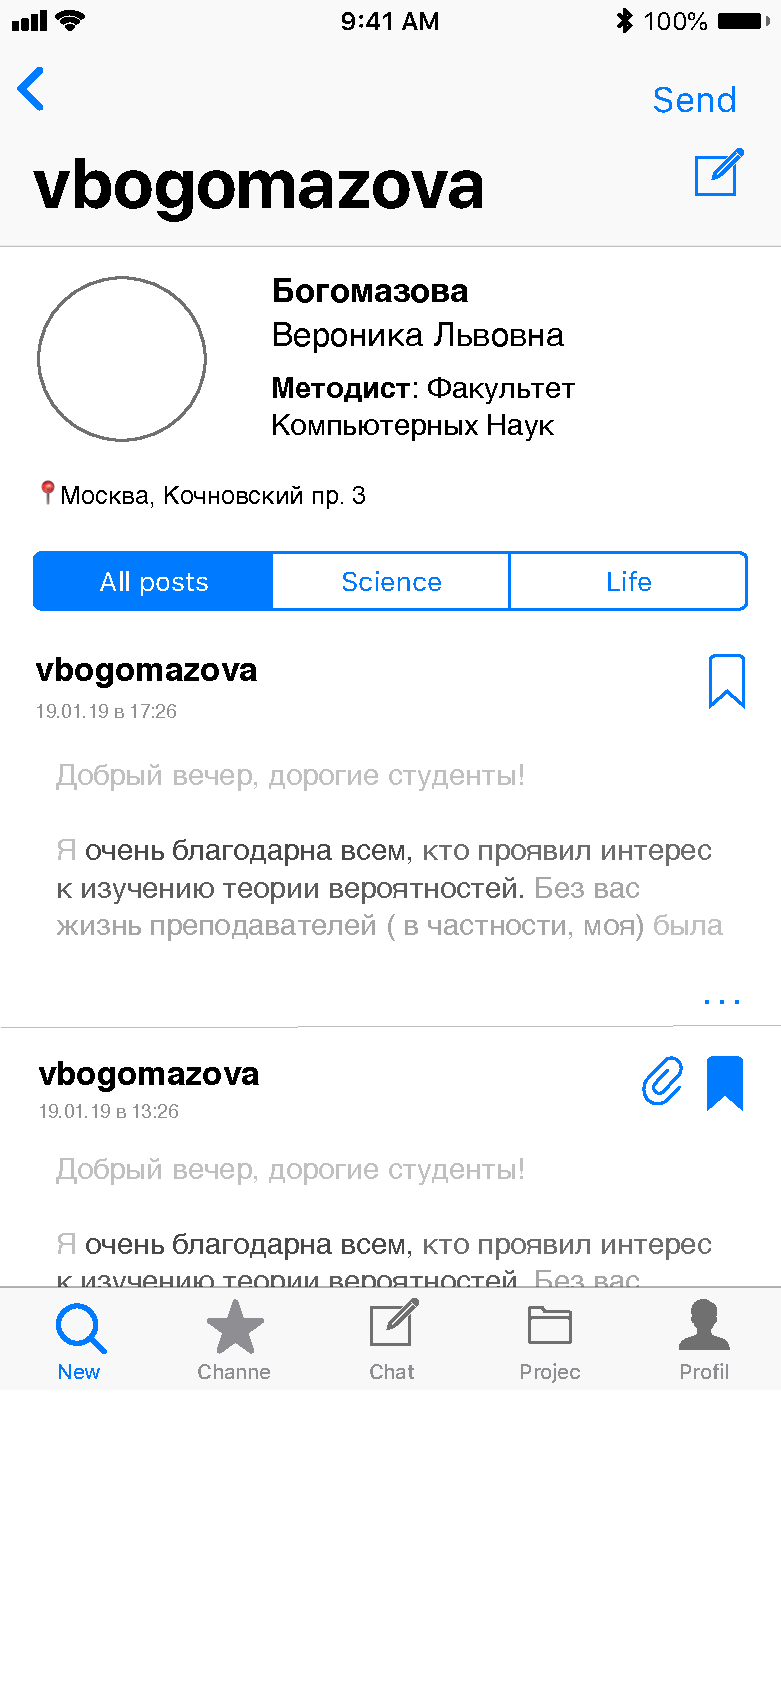
\includegraphics[width=\linewidth]{../includes/prototype/1.pdf}
		\end{subfigure}
		\begin{subfigure}[b]{0.3\linewidth}
			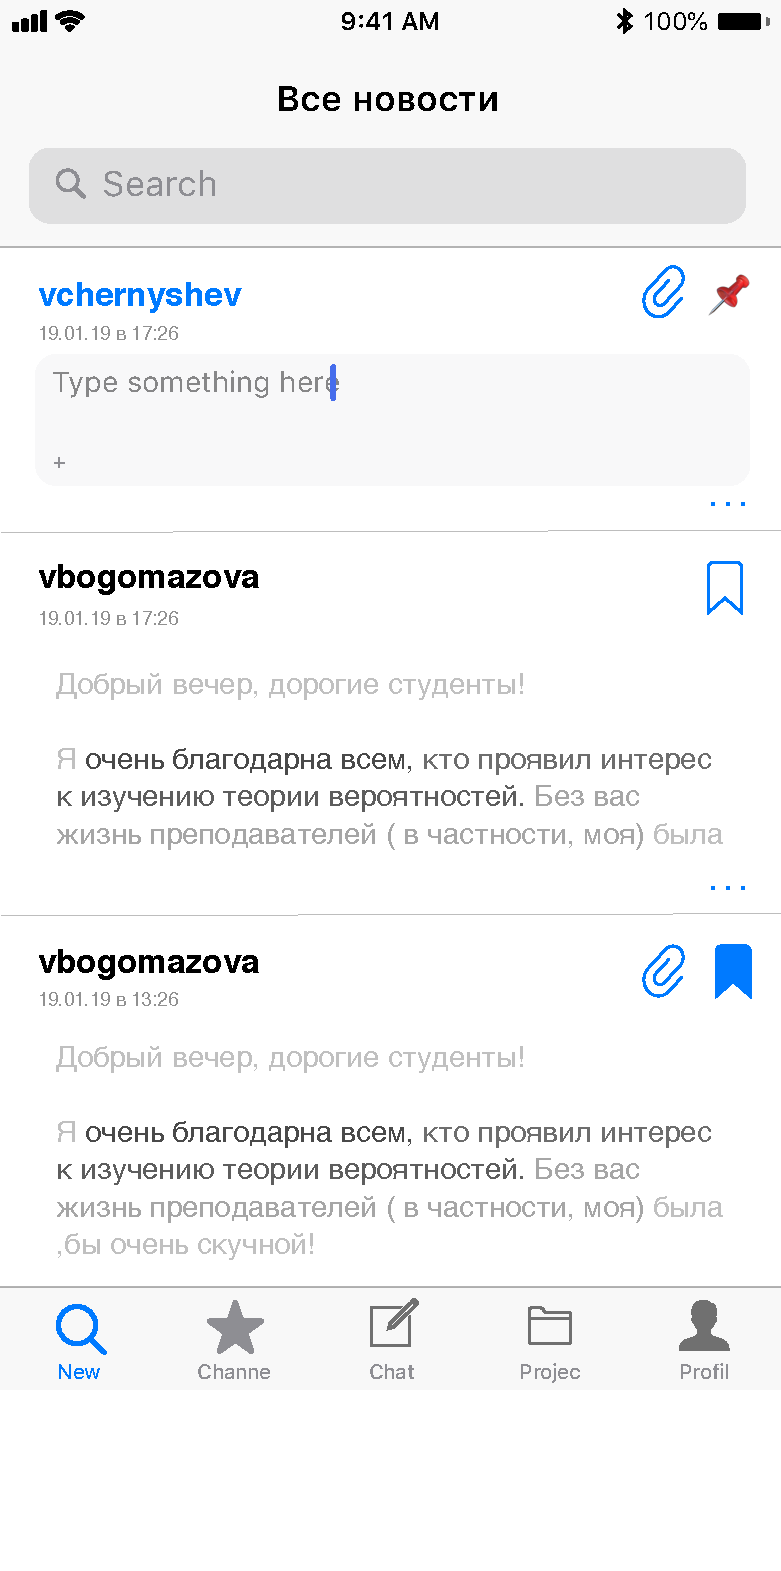
\includegraphics[width=\linewidth]{../includes/prototype/2.pdf}
		\end{subfigure}
		\begin{subfigure}[b]{0.3\linewidth}
			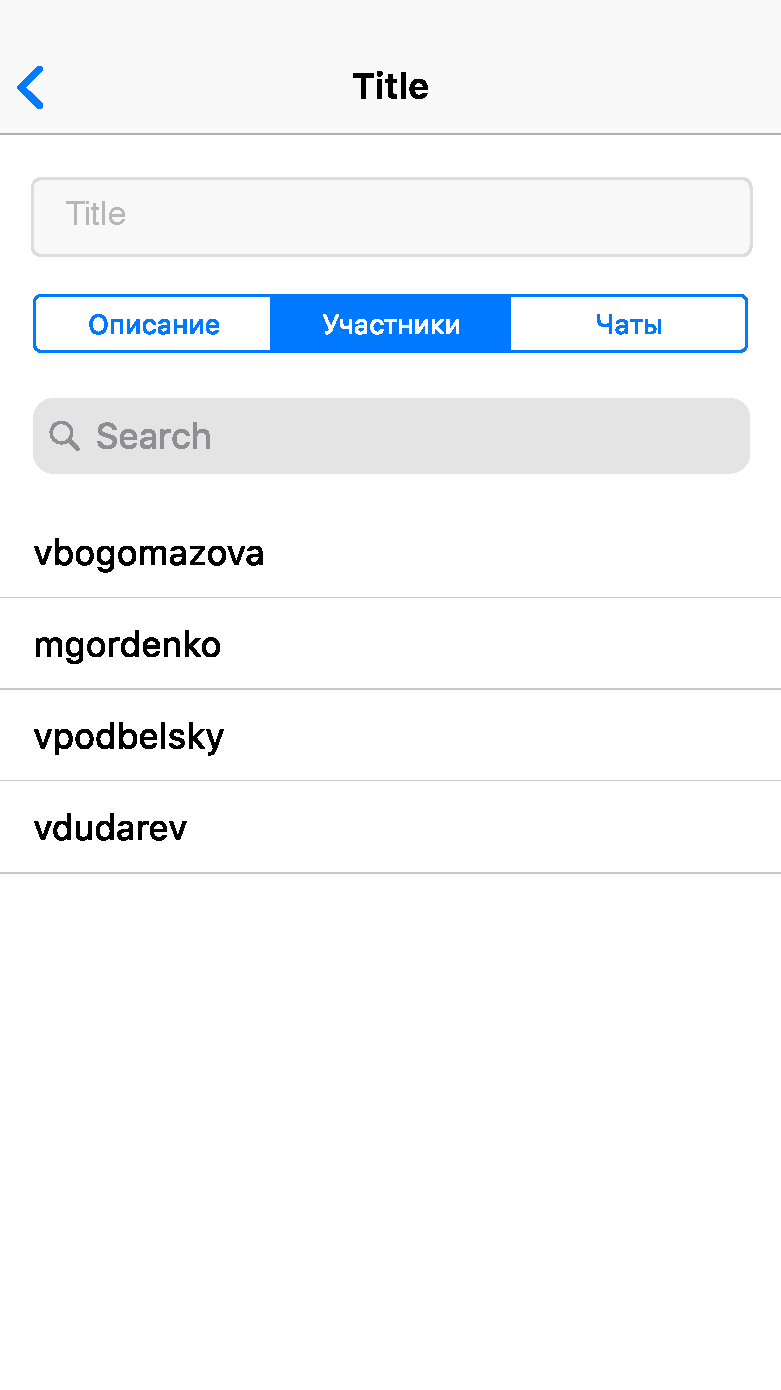
\includegraphics[width=\linewidth]{../includes/prototype/6.pdf}
		\end{subfigure}
		\begin{subfigure}[b]{0.3\linewidth}
			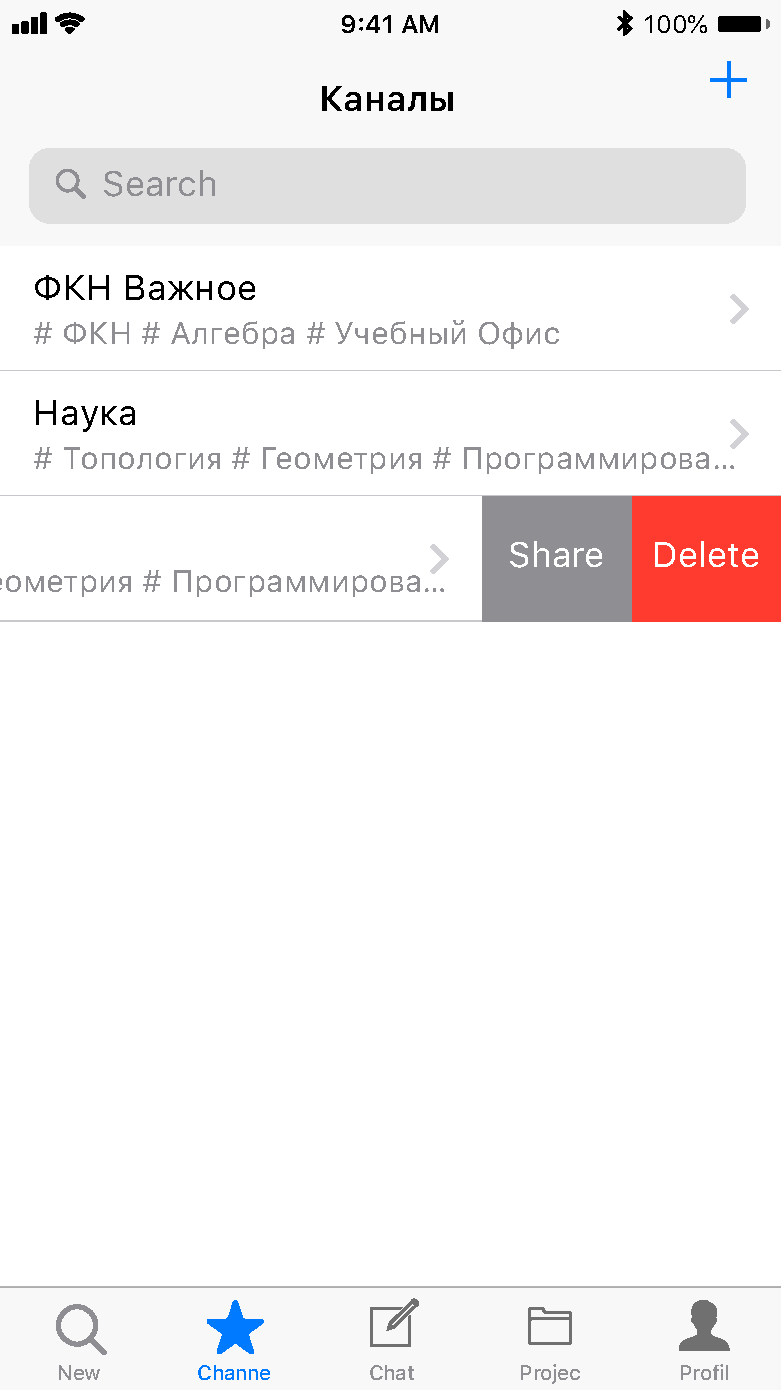
\includegraphics[width=\linewidth]{../includes/prototype/4.pdf}
		\end{subfigure}
		\begin{subfigure}[b]{0.3\linewidth}
			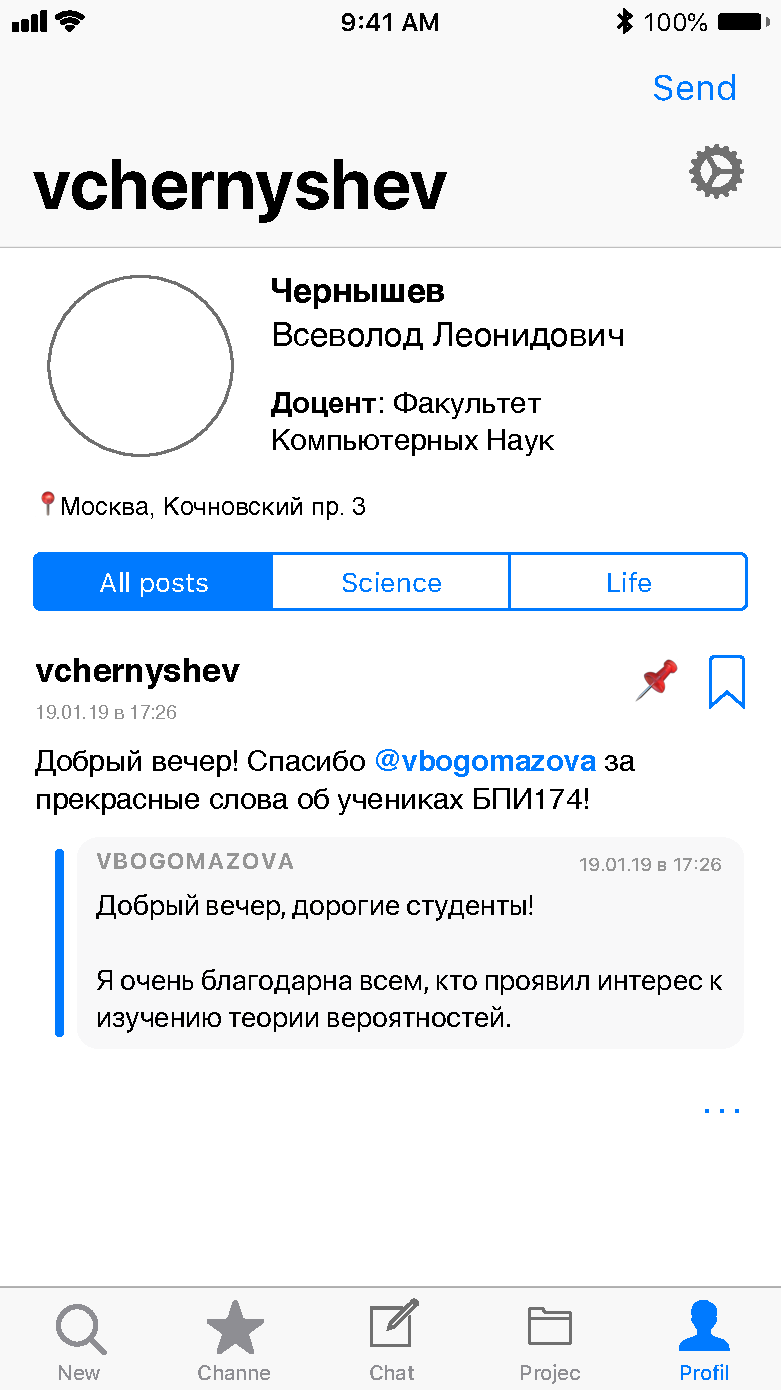
\includegraphics[width=\linewidth]{../includes/prototype/5.pdf}
		\end{subfigure}
		\begin{subfigure}[b]{0.3\linewidth}
			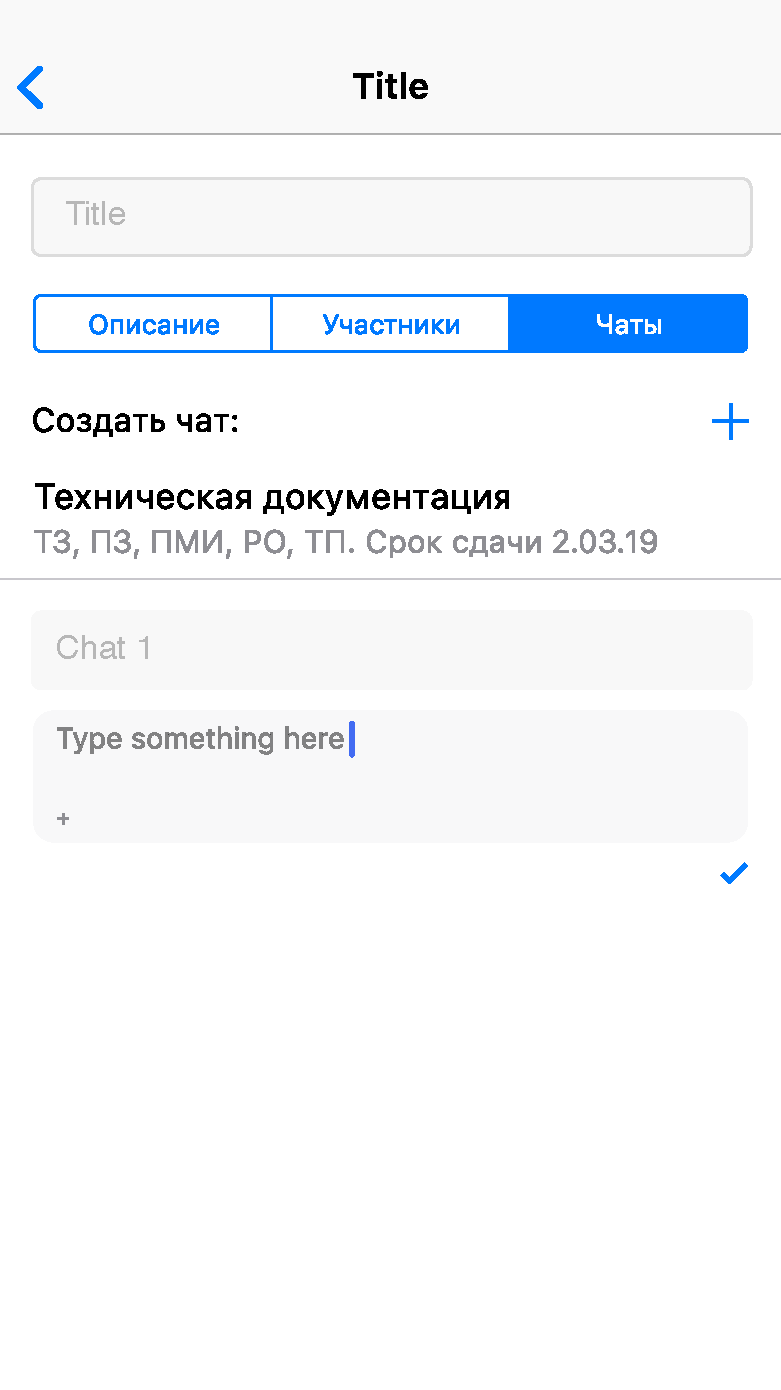
\includegraphics[width=\linewidth]{../includes/prototype/8.pdf}
		\end{subfigure}
		\caption{Прототип интерфейса}
	\end{figure}

	\newpage
	\addition{Статус требований}
	\begin{longtable}{|p{0.2\linewidth}|p{0.5\linewidth}|} 
	\caption{Статус требований} \label{statusReq} \\
\hline
\textbf{Proposed} & Требование запрошено авторизированным источником \\ \hline
\textbf{Approved} & Требование проанализировано, его влияние на проект просчитано, и оно было размещено в базовой версии определенной версии. \\ \hline
\textbf{Implemented} & Код, реализующий требование, разработан, написан и протестирован. Требование отслежено до соответствующих элементов дизайна и кода \\ \hline
\textbf{Verified} & Корректное функционирование реализованного требования подтверждено в соответствующем продукте. Требование отслежено до соответствующих вариантов тестирования. Теперь требование считается завершенным \\ \hline
\textbf{Deleted} & Утвержденное требование удалено из базовой версии.  \\ \hline
\textbf{Rejected} & Требование предложено, но не запланировано для реализации ни в одной будущих версий. \\ \hline

\end{longtable}

						\newpage
						
	\addition{SWOT-анализ} \label{addition: D}
	\begin{longtable}{|p{0.17\linewidth}|p{0.45\linewidth}|p{0.27\linewidth}|}
	\caption{SWOT-анализ} \label{swot} \\
    \hline 
    &  Позитивные& Негативные \\ 
    \hline 
    \textbf{Внутренние факторы}& {\footnotesize
       \begin{enumerate}
           \item Доступ исключительно для сотрудников ВШЭ
           \item Самое оптимальное решение для взаимодействия с научными публикациями
           \item Удобное взаимодействие между сотрудниками факультетов и кафедр
           \item Удобство публикаций научных работ преподавателями (аспирантами)
           \item Оперативное информирование сотрудников о достижениях коллег в интересующих их областях
           \item Быстрый поиск по интересующей области (статьи, рефераты, докторские и т.д.)
       \end{enumerate}
     }& {\footnotesize
       \begin{enumerate}
           \item Отсутствие сайта
           \item Отсутствие рекламной кампании
           \item Отсутствие десктопного приложения
           \item Отсутствие опыта в реализации подобных проектов
       \end{enumerate}
     } \\ 
    \hline 
    \textbf{Внешние факторы}& {\footnotesize
       \begin{enumerate}
           \item Открытие новых факультетов
           \item Увеличение штата сотрудников
           \item Сотрудничество с другими ВУЗами в сфере исследований
       \end{enumerate}
     }  & {\footnotesize
       \begin{enumerate}
           \item Проблемы с сервером
           \item Создание конкурентами лучшей социальной сети
           \item Незаинтересованность сотрудников
       \end{enumerate}
     } \\ 
    \hline 
\end{longtable} 
	\newpage
	%\section{Источники, использованные при разработке}
	%\renewcommand{\refname}{Список источников}
	% \addcontentsline{toc}{subsection}{\refname}
	\patchcmd{\thebibliography}{\section*{\refname}}{}{}{}
	\addition{Список источников}
	\begin{thebibliography}{6}
		\bibitem{interface} Human Interdace Guidelines [Электронный ресурс] URL: \url{https://developer.apple.com/design/human-interface-guidelines/ios/overview/themes} (Дата обращения: 16.05.2019, режим доступа: свободный)
		\bibitem{UIKit} UIKit [Электронный ресурс] URL: \url{https://developer.apple.com/documentation/uikit} (Дата обращения: 16.05.2019, режим доступа: свободный)
		\bibitem{gost}Единая система программной документации – М.: ИПК, Издательство стандартов, 2000, 125 стр.
		\bibitem{terms} Terms of use for Apple products [Электронный ресурс] URL: \url{https://www.apple.com/legal} (Дата обращения: 16.05.2019, режим доступа: свободный)
		\bibitem{lms} 
		LMS [Электронный ресурс] URL: 
		\url{https://lms.hse.ru} (Дата обращения: 16.05.2019, режим доступа: свободный)
		\bibitem{threads} 
		How to design social media interactions 
		[Электронный ресурс] URL:
		\url{https://medium.com/@michaelchaika/ho-to-design-social-media-interactions-386bdb5bee6d} (Дата обращения: 16.05.2019, режим доступа: свободный)
	\end{thebibliography}

						\newpage
	\listRegistration

\end{document} % конец документа